\documentclass[letterpaper,journal]{IEEEtran}

\usepackage{amsmath,amsfonts}
\usepackage{array}
\usepackage{booktabs}
\usepackage{cite}
\usepackage{graphicx}
\usepackage{siunitx}
\usepackage{url}

\hyphenation{comag-ne-to-meter magneto-enceph-alo-graphy}
\sisetup{detect-all}

\begin{document}

\title{Directional Shielding and Noise-Related Loss Characterization of Multilayer Thin-Ferrite Cylindrical Shields for Low-Noise Magnetic Instrumentation}

\author{Author~Name%
\thanks{Author affiliation, funding, and correspondence information should be added before submission.}
}

\markboth{IEEE Transactions on Instrumentation and Measurement}%
{Author: Multilayer Thin-Ferrite Cylindrical Shield Evaluation}

\maketitle

\begin{abstract}
Low-noise magnetic instruments are limited not only by sensor noise, but also by leakage fields and shield-related material-loss noise. This paper presents a measurement-oriented characterization method for multilayer thin-ferrite cylindrical shields. A no-shield directional reference is validated and used to calculate shielding factors from the intended magnetic-field component, while a separate virtual pickup-coil finite-element model provides the magnetic-noise-related loss indicator $\int H^2dV$ (IntH2) and its layer-resolved contributions. The method is applied to seven continuous-shell transverse-field candidates with \SI{100}{mm} inner radius, \SI{200}{mm} length, ferrite thickness from \SI{0.08}{mm} to \SI{0.60}{mm}, and screening material parameters $\mu_r'=1000$ and $\sigma=\SI{0.01}{S/m}$. The validated x-directed reference gives the expected vacuum field of approximately \SI{1.256637e-6}{T}; the seven transverse cases pass component-based $\mathrm{SF}_x$ processing and layerwise IntH2 summation checks. Mesh convergence is checked for the thinnest single-layer case and the selected four-layer case, although total-element, adaptive-pass, and air-domain-scale metadata remain unavailable in the present export. Among the equal-ferrite-volume continuous-shell candidates evaluated in the transverse field, the four-layer case gives the largest $\mathrm{SF}_x$ and the lowest IntH2-normalized auxiliary loss indices. The present conclusions are limited to validated transverse continuous-shell simulations and do not constitute a final instrument-level recommendation.
\end{abstract}

\begin{IEEEkeywords}
Ferrite magnetic shield, finite-element method, instrumentation, magnetic noise, multilayer cylindrical shell, shielding factor.
\end{IEEEkeywords}

\section{Introduction}
\IEEEPARstart{U}{ltra-sensitive} magnetic measurement systems, including atomic magnetometers, spin-exchange-relaxation-free (SERF) comagnetometers, magnetoencephalography instruments, and precision tests of fundamental symmetries, require a controlled low-field and low-noise magnetic environment \cite{ref1,ref2,ref3,ref4,ref5}. In such systems, the magnetic shield is part of the measurement chain. It determines the environmental-field leakage that reaches the sensor and can also generate magnetic-field noise through material loss. Therefore, the shield should not be evaluated only by a single shielding factor. For low-noise magnetic instrumentation, directional shielding factor, center leakage field, ferrite volume, radial space occupation, and material-loss-related noise indicators should be evaluated together.

High-permeability metallic shields are widely used to attenuate static and low-frequency fields \cite{ref6,ref7,ref8}. However, their high electrical conductivity produces eddy-current magnetic noise that can become relevant in the frequency band of high-sensitivity magnetometers \cite{ref9,ref10,ref11}. Ferrites are attractive alternatives because their conductivity is much lower than that of metallic alloys. This suppresses eddy-current noise; the remaining low-frequency shield-induced noise is then associated mainly with magnetic loss, represented by the imaginary permeability $\mu_r''$, and with the spatial distribution of magnetic field inside the ferrite \cite{ref9,ref12,ref13,ref14,ref15}. A recent IEEE TIM study on cubic ferrite shields demonstrated the practical importance of ferrites in compact low-noise shielding \cite{ref16}. Nevertheless, the cubic panel geometry does not directly address open-ended cylindrical shields, which are common around atomic sensors and compact comagnetometers.

A monolithic cylindrical ferrite shield is mechanically difficult to fabricate when the diameter is large and the wall is thin. Ferrites are brittle after sintering, and machining a \SI{200}{mm}-diameter thin-walled cylinder with sub-millimeter wall thickness is costly and fragile. A manufacturable alternative is to assemble a shield from multilayer thin-ferrite cylindrical shells or segmented ferrite sheets. This introduces a coupled design problem: layer number $N_L$, ferrite thickness $a$, radial gap $g$, circumferential segmentation, ferrite volume $V_f$, and total radial occupation all affect the center leakage field and the geometry-dependent loss integral used in magnetic-noise calculations.

Existing studies provide important foundations, but do not fully cover this measurement-oriented design problem. Kornack \textit{et al.} reported a low-noise ferrite cylinder with measured magnetic noise \cite{ref12}. Lee and Romalis derived magnetic-noise formulas for high-permeability shields and conducting objects with simple geometry \cite{ref9}. Later studies modeled cylindrical or multi-annular ferrite shields and discussed gap effects and material parameters \cite{ref13,ref14,ref17}. However, previous work has not simultaneously reported a validated no-shield directional reference, layer-resolved IntH2 analysis, and a multilayer thin-ferrite cylindrical geometry under a unified evaluation framework. Table~\ref{tab:comparison} summarizes the relationship between representative prior work and the present manuscript.

\begin{table*}[!t]
\caption{Relationship to Representative Ferrite Shield Studies}
\label{tab:comparison}
\centering
\footnotesize
\setlength{\tabcolsep}{3pt}
\begin{tabular}{p{0.16\textwidth}p{0.18\textwidth}p{0.18\textwidth}p{0.32\textwidth}}
\toprule
Work & Geometry & Main quantity & Scope relative to this work \\
\midrule
Kornack \textit{et al.} \cite{ref12} & Single ferrite cylinder & SF and measured noise & No multilayer thin-shell comparison \\
Lee and Romalis \cite{ref9} & Simple analytic shapes & Magnetic-noise formula & No finite-length multilayer FEM geometry \\
Ma \textit{et al.} \cite{ref13} & Cylindrical ferrite shield & SF and IntH2 & Layer-resolved IntH2 not reported \\
Lu \textit{et al.} \cite{ref14,ref17} & Multi-annular/gapped ferrite shields & Noise-related FEM analysis & Directional no-shield reference not emphasized \\
Sun \textit{et al.} \cite{ref16} & Cubic ferrite shield & SF and measured noise & Cubic geometry, not cylindrical multilayer shell \\
This work & Multilayer thin-ferrite cylinder & Directional SF, $V_f$, layerwise IntH2 & Measurement-oriented characterization method with validation studies \\
\bottomrule
\end{tabular}
\end{table*}

The novelty of this work is not simply the use of multiple ferrite layers. The contribution is a measurement-oriented characterization method rather than a final instrument-level shield recommendation. It combines: 1) validated no-shield directional references for component-based shielding-factor evaluation; 2) a virtual pickup-coil model for the geometry-dependent magnetic-noise-related loss integral; 3) layer-resolved IntH2 decomposition for multilayer shields; 4) fixed-volume comparison between single-layer and multilayer candidates; 5) unit-consistent auxiliary metrics for low-noise shield design; and 6) validation-gated reporting so that missing or planned studies are not converted into conclusions.

\section{Measurement-Oriented Characterization Principle}

\subsection{Coordinate System and Measurement Configuration}

The shield is modeled as a device under test (DUT) placed at the center of a calibrated magnetic-field region. The cylinder axis is defined as the Cartesian $z$-axis, while $x$ and $y$ span the transverse plane. Because the shield is a finite open-ended cylinder, transverse and axial shielding are not equivalent. The quantities $\mathrm{SF}_x$ and $\mathrm{SF}_y$ describe transverse shielding through the sidewall, whereas $\mathrm{SF}_z$ describes axial shielding affected by leakage through the open ends \cite{ref6,ref27,ref28,ref29}.

Two finite-element models are used, as shown schematically in Fig.~\ref{fig:framework}. These models answer different measurement questions and should not be physically conflated. The external uniform-field model evaluates environmental-field attenuation and provides $B_0$, $B_{\mathrm{center}}$, $\mathrm{SF}_q$, and $\mathrm{LeakageRatio}_q$. The virtual pickup-coil model evaluates how material loss couples to the measured magnetic field through the fluctuation-dissipation theorem and provides $\mathrm{IntH2}_{\mathrm{total}}$ and $\mathrm{IntH2}_{L_i}$.

\begin{figure}[!t]
\centering
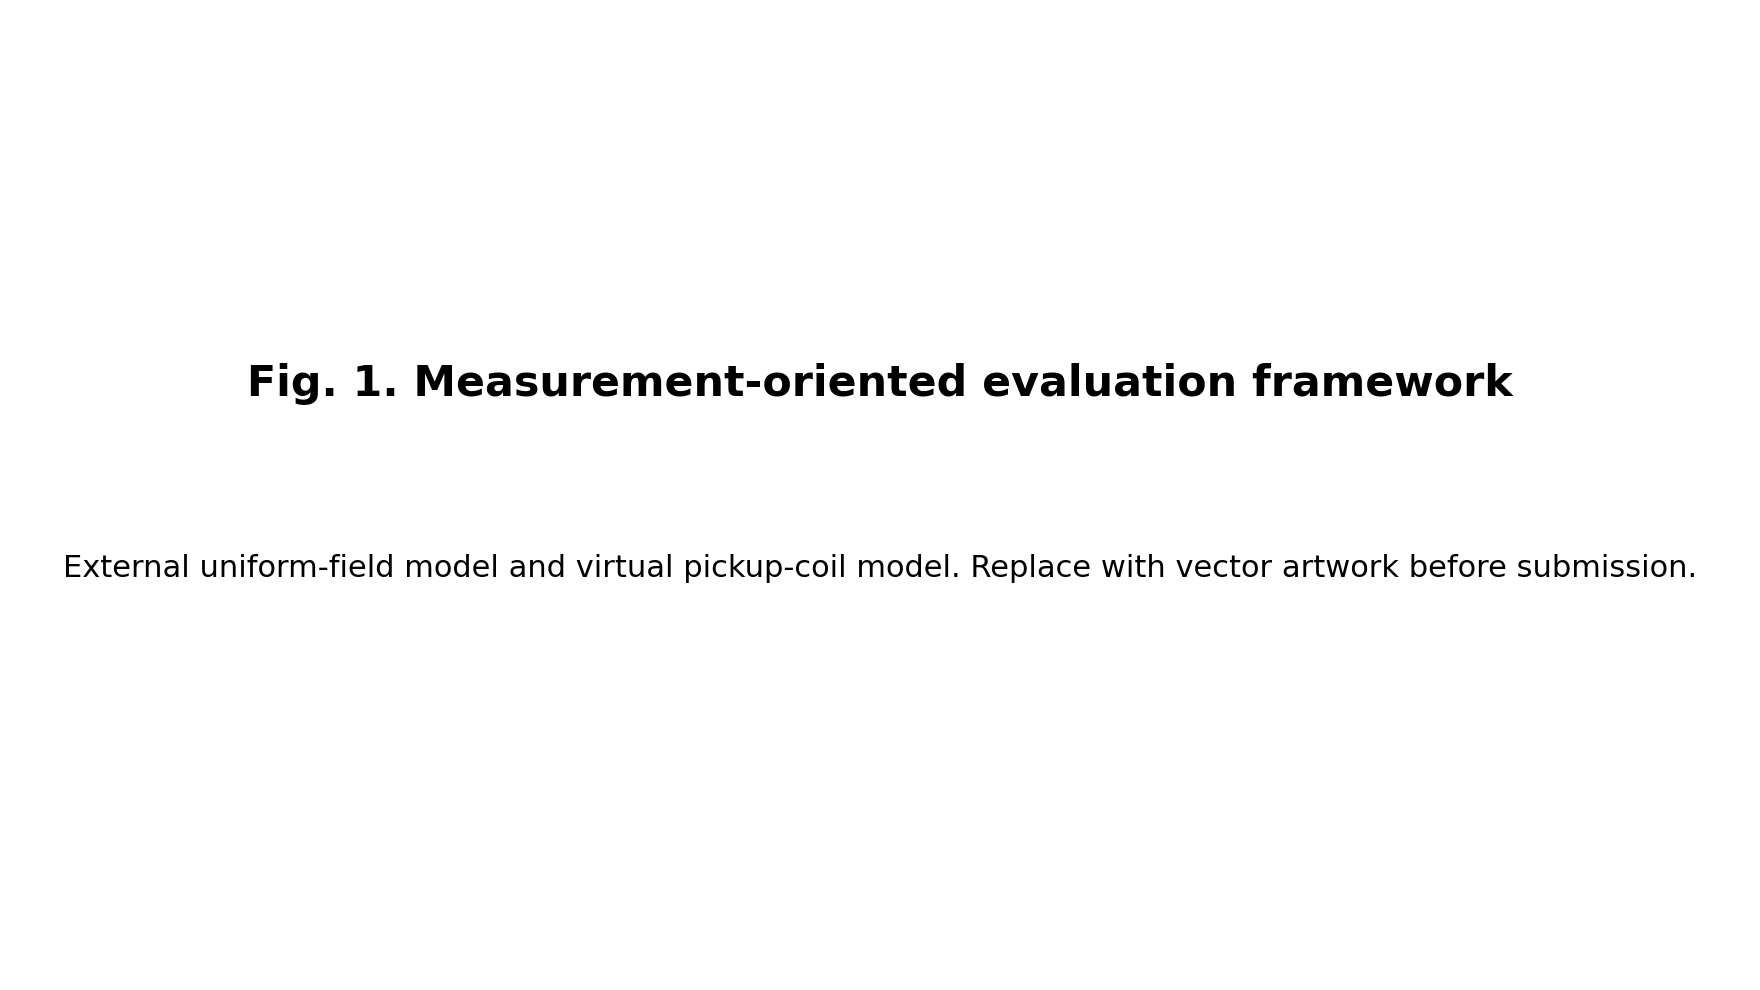
\includegraphics[width=\columnwidth]{../figures/Fig1_measurement_framework.png}
\caption{Measurement-oriented characterization principle. The external uniform-field problem provides $B_0$, $B_{\mathrm{center}}$, $\mathrm{SF}_q$, and $\mathrm{LeakageRatio}_q$; the virtual pickup-coil problem provides IntH2 and layer-resolved IntH2.}
\label{fig:framework}
\end{figure}

\subsection{Directional Shielding Factor}

For an external field applied along $q\in\{x,y,z\}$, the no-shield reference field at the observation point is
\begin{equation}
\mathbf{B}_0=(B_{0,x},B_{0,y},B_{0,z}),
\label{eq:B0}
\end{equation}
and the shielded center leakage field is
\begin{equation}
\mathbf{B}_{\mathrm{center}}=(B_{\mathrm{center},x},B_{\mathrm{center},y},B_{\mathrm{center},z}).
\label{eq:Bcenter}
\end{equation}
The directional shielding factor is defined by
\begin{equation}
\mathrm{SF}_q=\frac{|B_{0,q}|}{|B_{\mathrm{center},q}|},
\label{eq:sfq}
\end{equation}
and the corresponding leakage ratio is
\begin{equation}
\mathrm{LeakageRatio}_q=\frac{|B_{\mathrm{center},q}|}{|B_{0,q}|}=\frac{1}{\mathrm{SF}_q}.
\label{eq:leakage}
\end{equation}
The formal shielding factor is computed from the intended directional component. The vector magnitude $B_{\mathrm{Mag}}$ is retained only as an auxiliary consistency check and is not used as the primary SF definition.

\subsection{No-Shield Directional Reference}

The no-shield model is the calibration reference for the external-field problem. The ferrite bodies are deleted or assigned vacuum while the air region, boundary dimensions, observation point, solver setting, and excitation amplitude are kept identical to the shielded model. In vacuum, for $H_0=\SI{1}{A/m}$,
\begin{equation}
B_0=\mu_0 H_0=(4\pi\times10^{-7})(1)=1.256637\times10^{-6}\ \mathrm{T}.
\label{eq:vacuum}
\end{equation}
Thus, an ideal $x$-directed reference should give $B_{0,x}\approx\SI{1.256637e-6}{T}$, with $B_{0,y}$ and $B_{0,z}$ much smaller. The residual transverse components are treated as numerical residuals caused by finite-element discretization, finite-domain boundary approximation, and interpolation at the observation point.

The reference field is accepted only if the intended component dominates the other components:
\begin{equation}
\Gamma_q=\frac{|B_{0,q}|}{\max_{p\ne q}|B_{0,p}|}.
\label{eq:purity}
\end{equation}
In the post-processing rule set, a failed directional reference prevents the corresponding shielding factors from being used in figures or conclusions.

\subsection{Analytical Scaling Motivation}

The finite-element model is the primary evaluation tool because the shield is finite in length, open ended, and may include layer gaps or segmented slots. Nevertheless, the choice of design variables is guided by the classical transverse cylindrical-shell solution. In a source-free region with linear isotropic permeability, $\nabla\times\mathbf{H}=0$ and $\nabla\cdot\mathbf{B}=0$ allow the magnetic scalar potential to satisfy Laplace's equation. For an infinitely long coaxial cylindrical shell in a transverse uniform field, the potential in each annular region can be written as
\begin{equation}
\phi_k(r,\theta)=\left(C_k r+\frac{D_k}{r}\right)\cos\theta ,
\label{eq:scalarpotential}
\end{equation}
where the constants are obtained from the continuity of normal $B$ and tangential $H$ at each interface \cite{ref6}. For a single high-permeability thin shell, this solution gives the familiar leading transverse scaling
\begin{equation}
S_T \simeq 1+\frac{\mu_r t}{2R},
\label{eq:singlelayerscaling}
\end{equation}
showing that shell thickness, mean radius, and permeability set the first-order shielding contribution.

For a multilayer coaxial shell, the analytical expansion contains direct layer terms and interlayer radius-coupling terms. A typical coupling factor between two layers with mean radii $R_i<R_j$ is
\begin{equation}
\Lambda_{ij}=1-\left(\frac{R_i}{R_j}\right)^2 .
\label{eq:couplingfactor}
\end{equation}
This motivates comparing layer number, radial gap, and total radial occupation rather than comparing total thickness alone. The present manuscript uses this analytical structure only as a scaling motivation; the reported $\mathrm{SF}_q$ values are obtained from the validated directional FEM reference in (\ref{eq:sfq}), not from the ideal infinite-cylinder expression.

Under the thin-shell approximation, a set of equal-height coaxial layers with total ferrite thickness $T_f=N_La$ has
\begin{equation}
V_f\approx 2\pi L R_c T_f ,
\label{eq:vfapprox}
\end{equation}
where $R_c$ is the radial-window center radius. Therefore, fixed $T_f$ is a useful first-order proxy for fixed ferrite volume. In the actual post-processing, however, $V_f$ is always computed from the exact layer radii in (\ref{eq:vf}) or from CAD volume export.

\subsection{Virtual Pickup-Coil Model and IntH2}

The shield-induced magnetic noise can be related to material loss through the fluctuation-dissipation theorem \cite{ref9,ref18}. A virtual pickup coil placed at the observation point produces a magnetic field $H_{\mathrm{vc}}$ in the ferrite. For coil area $A$, turn number $N_c$, peak current $I_0$, and magnetic moment $m=AN_cI_0$, the hysteresis-loss contribution to the magnetic-field noise amplitude spectral density can be written as
\begin{equation}
\delta B_{\mathrm{hyst}}(f)=
\frac{1}{m}
\left(
\frac{2k_{\mathrm{B}}T\mu''}{\pi f}
\int_V H_{\mathrm{vc}}^2\,dV
\right)^{1/2},
\label{eq:noisemodel}
\end{equation}
where $\mu''=\mu_0\mu_r''$ is the absolute imaginary permeability if $\mu_r''$ is specified as a relative quantity. The current $I_0$ is a peak current; if an RMS current is used in another implementation, the normalization must be converted consistently.

This manuscript does not claim measured magnetic-noise spectra. The exported FEM quantity is the geometry-dependent magnetic-noise-related loss indicator
\begin{equation}
\mathrm{IntH2}=\int_V H_{\mathrm{vc}}^2\,dV,
\label{eq:inth2}
\end{equation}
with SI unit $\mathrm{A^2\,m}$. IntH2 becomes an absolute noise prediction only after measured $\mu_r''(f)$, temperature, frequency, and virtual-coil normalization are specified. Relative comparison by IntH2 is meaningful only for identical material properties, identical coil normalization, and identical observation direction.

For two candidate geometries $A$ and $B$ evaluated under identical material loss and virtual-coil normalization, (\ref{eq:noisemodel}) gives the relative loss-induced field-noise scaling
\begin{equation}
\frac{\delta B_A(f)}{\delta B_B(f)}
=
\left(
\frac{\mathrm{IntH2}_A}{\mathrm{IntH2}_B}
\right)^{1/2}.
\label{eq:relnoise}
\end{equation}
Thus, IntH2 ratios should not be interpreted linearly as magnetic-noise ratios; the square-root relation applies only under the identical-normalization assumptions stated above.

For a multilayer shield, each ferrite layer is retained as an independent body. The layer-resolved terms are
\begin{equation}
\mathrm{IntH2}_{L_i}=\int_{V_{L_i}}H_{\mathrm{vc}}^2\,dV,
\label{eq:inth2layer}
\end{equation}
and
\begin{equation}
\mathrm{IntH2}_{\mathrm{total}}=\sum_{i=1}^{N_L}\mathrm{IntH2}_{L_i}.
\label{eq:inth2total}
\end{equation}
The export is accepted only if
\begin{equation}
\frac{|\mathrm{IntH2}_{\mathrm{total}}-\sum_i\mathrm{IntH2}_{L_i}|}
{|\mathrm{IntH2}_{\mathrm{total}}|}<10^{-3}.
\label{eq:inth2check}
\end{equation}

\section{FEM Implementation and Data Processing}

\subsection{Multilayer Cylindrical Geometry}

The DUT is an open-ended multilayer cylindrical shell with inner radius $R_{\mathrm{in}}$, axial length $L$, layer count $N_L$, ferrite thickness $a$, and radial interlayer gap $g$. The current design matrix uses
\begin{equation}
R_{\mathrm{in}}=\SI{100}{mm},\qquad L=\SI{200}{mm}.
\label{eq:basicgeometry}
\end{equation}
The total ferrite thickness and radial occupation are
\begin{equation}
T_f=N_La,
\label{eq:tf}
\end{equation}
\begin{equation}
T_{\mathrm{space}}=N_La+(N_L-1)g.
\label{eq:tspace}
\end{equation}
For layer $i$, where $i=1$ is the innermost layer,
\begin{align}
R_{i,\mathrm{in}} &= R_{\mathrm{in}}+(i-1)(a+g),\\
R_{i,\mathrm{out}} &= R_{i,\mathrm{in}}+a.
\end{align}
The ferrite volume is calculated from the exact cylindrical-shell expression
\begin{equation}
V_f=\pi L\sum_{i=1}^{N_L}\left(R_{i,\mathrm{out}}^2-R_{i,\mathrm{in}}^2\right).
\label{eq:vf}
\end{equation}
Although $V_f$ is displayed in $\mathrm{mm^3}$ for engineering readability, all SI-derived metrics are computed after unit conversion.

For segmented-shell correction, the circumferential coverage fraction is defined as
\begin{equation}
\eta_\phi=1-\frac{N_{\mathrm{seg}}g_\phi}{2\pi R_{\mathrm{mid}}},
\label{eq:etaphi}
\end{equation}
where $N_{\mathrm{seg}}$ is the number of circumferential segments, $g_\phi$ is the slot width, and $R_{\mathrm{mid}}$ is the layer mid-radius. Aligned and staggered slot patterns are evaluated separately when the segmented AEDT models are available.

\begin{figure}[!t]
\centering
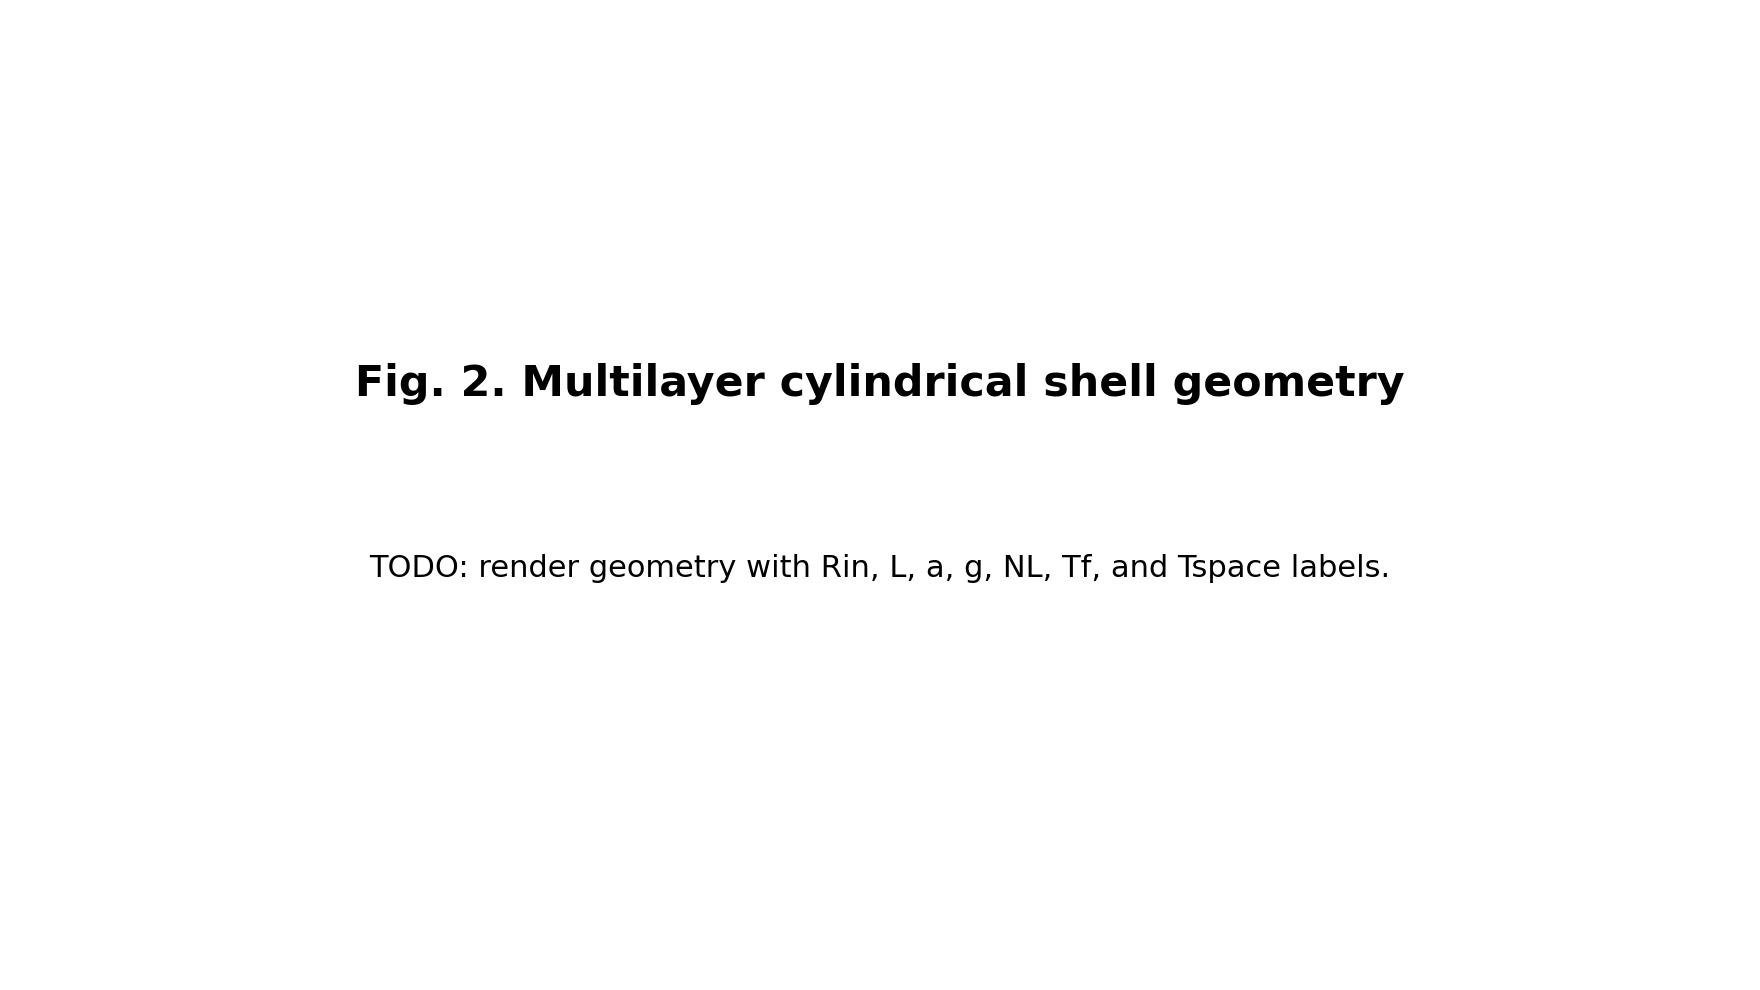
\includegraphics[width=\columnwidth]{../figures/Fig2_multilayer_cylindrical_geometry.png}
\caption{Geometry definition for the multilayer thin-ferrite cylindrical shell.}
\label{fig:geometry}
\end{figure}

\subsection{Simulation Matrix and Data Export}

The present main matrix is a transverse continuous-shell screening study. It is intentionally separated from axial, segmented, permeability-sensitivity, and convergence studies so that each validation stage can be tracked independently. Table~\ref{tab:matrix} lists the current main cases.

\begin{table*}[!t]
\caption{Main Continuous-Shell Transverse Matrix}
\label{tab:matrix}
\centering
\footnotesize
\setlength{\tabcolsep}{3pt}
\begin{tabular}{p{0.24\textwidth}ccccp{0.32\textwidth}}
\toprule
Case & $N_L$ & $a$ (mm) & $g$ (mm) & Direction & Purpose \\
\midrule
B0\_reference\_x & 0 & 0 & 0 & $x$ & no-shield reference \\
C1\_N1\_t008\_x & 1 & 0.08 & 0 & $x$ & thinnest single layer \\
C1\_N1\_t020\_x & 1 & 0.20 & 0 & $x$ & thin single layer \\
C1\_N1\_t040\_x & 1 & 0.40 & 0 & $x$ & intermediate single layer \\
C1\_N1\_t060\_x & 1 & 0.60 & 0 & $x$ & equal-volume single-layer baseline \\
C2\_N2\_t020\_g010\_x & 2 & 0.20 & 0.10 & $x$ & multilayer candidate \\
C2\_N3\_t020\_g010\_x & 3 & 0.20 & 0.10 & $x$ & equal-volume multilayer candidate \\
C2\_N4\_t015\_g008\_x & 4 & 0.15 & 0.08 & $x$ & equal-volume multilayer candidate \\
\bottomrule
\end{tabular}
\end{table*}

Each shielded external-field case exports $B_{\mathrm{center},x}$, $B_{\mathrm{center},y}$, $B_{\mathrm{center},z}$, and $B_{\mathrm{center,Mag}}$. The no-shield reference exports $B_{0,x}$, $B_{0,y}$, $B_{0,z}$, and $B_{0,\mathrm{Mag}}$. Each virtual pickup-coil case exports $\mathrm{IntH2}_{\mathrm{total}}$ and the layerwise quantities $\mathrm{IntH2}_{L_i}$. The post-processing scripts merge raw CSV exports by case ID and field direction, compute the derived metrics, and mark missing or failed rows without substituting zero values.

\subsection{Comparison Metrics}

The volume-normalized shielding index is defined as
\begin{equation}
\eta_S=\frac{\ln(\mathrm{SF}_x)}{V_f}.
\label{eq:etas}
\end{equation}
It is an auxiliary index introduced for this comparison, not a material property. When $V_f$ is reported in $\mathrm{mm^3}$, the displayed unit is $\mathrm{mm^{-3}}$; SI-derived quantities are computed after converting volume to $\mathrm{m^3}$.

A dimensionless normalized form is
\begin{equation}
\eta_S^*=
\frac{\ln(\mathrm{SF}_x)/V_f}{\ln(\mathrm{SF}_{x,\mathrm{ref}})/V_{\mathrm{ref}}},
\label{eq:etasstar}
\end{equation}
where the reference is the continuous single-layer shell with $a=\SI{0.60}{mm}$. The loss-integral density and attenuation-normalized loss indicator are
\begin{equation}
\rho_H=\frac{\mathrm{IntH2}_{\mathrm{total}}}{V_f[\mathrm{m^3}]},
\label{eq:rhoh}
\end{equation}
\begin{equation}
\chi_H=\frac{\mathrm{IntH2}_{\mathrm{total}}}{\ln(\mathrm{SF}_x)}.
\label{eq:chih}
\end{equation}
The metrics are interpreted jointly with $T_{\mathrm{space}}$ and the validation status. No single auxiliary metric defines a final shield geometry.

\subsection{Paper-Use Consistency Rules}

Only validated rows are used in the Results section. A row is eligible if the corresponding raw export is present, the B0 direction check has passed, the directional field component needed for $\mathrm{SF}_q$ is present, the layerwise IntH2 check has passed when layerwise IntH2 is used, and the row is not marked planned, missing, pending, or failed. The vector magnitude $B_{\mathrm{Mag}}$ is never used as the formal shielding-factor denominator or numerator.

\subsection{Prototype Measurement Status}

No prototype shielding-factor measurement is reported in this paper. A concise measurement note is provided in Appendix~\ref{app:prototype} only to keep the FEM definitions traceable to a future experiment; it is not used as validation evidence.

\section{Results}

\subsection{Directional Reference Validation}

Table~\ref{tab:b0validation} shows the component-level validation of the no-shield reference models. Both x- and z-directed references passed the direction-purity check. The x-directed reference is therefore used for the transverse shielding-factor calculations in this paper. The z-directed reference is accepted as the axial no-shield reference, but no axial shielded result is reported unless the corresponding shielded z-directed raw export is present and validated.

\begin{table}[!t]
\caption{No-Shield Directional Reference Validation}
\label{tab:b0validation}
\centering
\footnotesize
\setlength{\tabcolsep}{2.5pt}
\begin{tabular}{lccccc}
\toprule
Reference & Dir. & $|B_x|$ & $|B_y|$ & $|B_z|$ & Status \\
 & & (T) & (T) & (T) & \\
\midrule
B0\_reference\_x & x & 1.257e-6 & 3.828e-15 & 1.943e-13 & passed \\
B0\_reference\_z & z & 2.468e-15 & 3.361e-14 & 1.257e-6 & passed \\
\bottomrule
\end{tabular}
\end{table}

\subsection{Transverse Continuous-Shell Characterization}

Seven x-directed continuous-shell cases satisfy the data-use rules. Table~\ref{tab:transverseresults} lists their processed results, and Fig.~\ref{fig:sfxvf} shows $\mathrm{SF}_x$ versus ferrite volume. The single-layer cases show increasing $\mathrm{SF}_x$ with thickness under the tested transverse condition. The multilayer cases are compared using the same directional B0 reference and the same screening material parameters.

\begin{table*}[!t]
\caption{Validated Transverse Continuous-Shell Results}
\label{tab:transverseresults}
\centering
\footnotesize
\setlength{\tabcolsep}{2.5pt}
\begin{tabular}{lccccccccc}
\toprule
Case & $N_L$ & $a$ & $g$ & $V_f$ & $T_{\mathrm{space}}$ & $B_{\mathrm{center},x}$ & $\mathrm{SF}_x$ & Leakage & IntH2 \\
 & & (mm) & (mm) & (mm$^3$) & (mm) & (T) & & ratio & (A$^2$m) \\
\midrule
C1\_N1\_t008\_x & 1 & 0.08 & 0.00 & 10057.1 & 0.08 & 9.375e-7 & 1.340 & 0.746 & 3.819e-6 \\
C1\_N1\_t020\_x & 1 & 0.20 & 0.00 & 25157.9 & 0.20 & 8.353e-7 & 1.504 & 0.665 & 4.383e-6 \\
C1\_N1\_t040\_x & 1 & 0.40 & 0.00 & 50366.0 & 0.40 & 5.832e-7 & 2.155 & 0.464 & 4.973e-6 \\
C1\_N1\_t060\_x & 1 & 0.60 & 0.00 & 75624.4 & 0.60 & 4.418e-7 & 2.845 & 0.352 & 4.649e-6 \\
C2\_N2\_t020\_g010\_x & 2 & 0.20 & 0.10 & 50391.1 & 0.50 & 5.616e-7 & 2.238 & 0.447 & 4.917e-6 \\
C2\_N3\_t020\_g010\_x & 3 & 0.20 & 0.10 & 75699.8 & 0.80 & 4.197e-7 & 2.994 & 0.334 & 4.381e-6 \\
C2\_N4\_t015\_g008\_x & 4 & 0.15 & 0.08 & 75714.9 & 0.84 & 3.463e-7 & 3.629 & 0.276 & 4.160e-6 \\
\bottomrule
\end{tabular}
\end{table*}

\begin{figure}[!t]
\centering
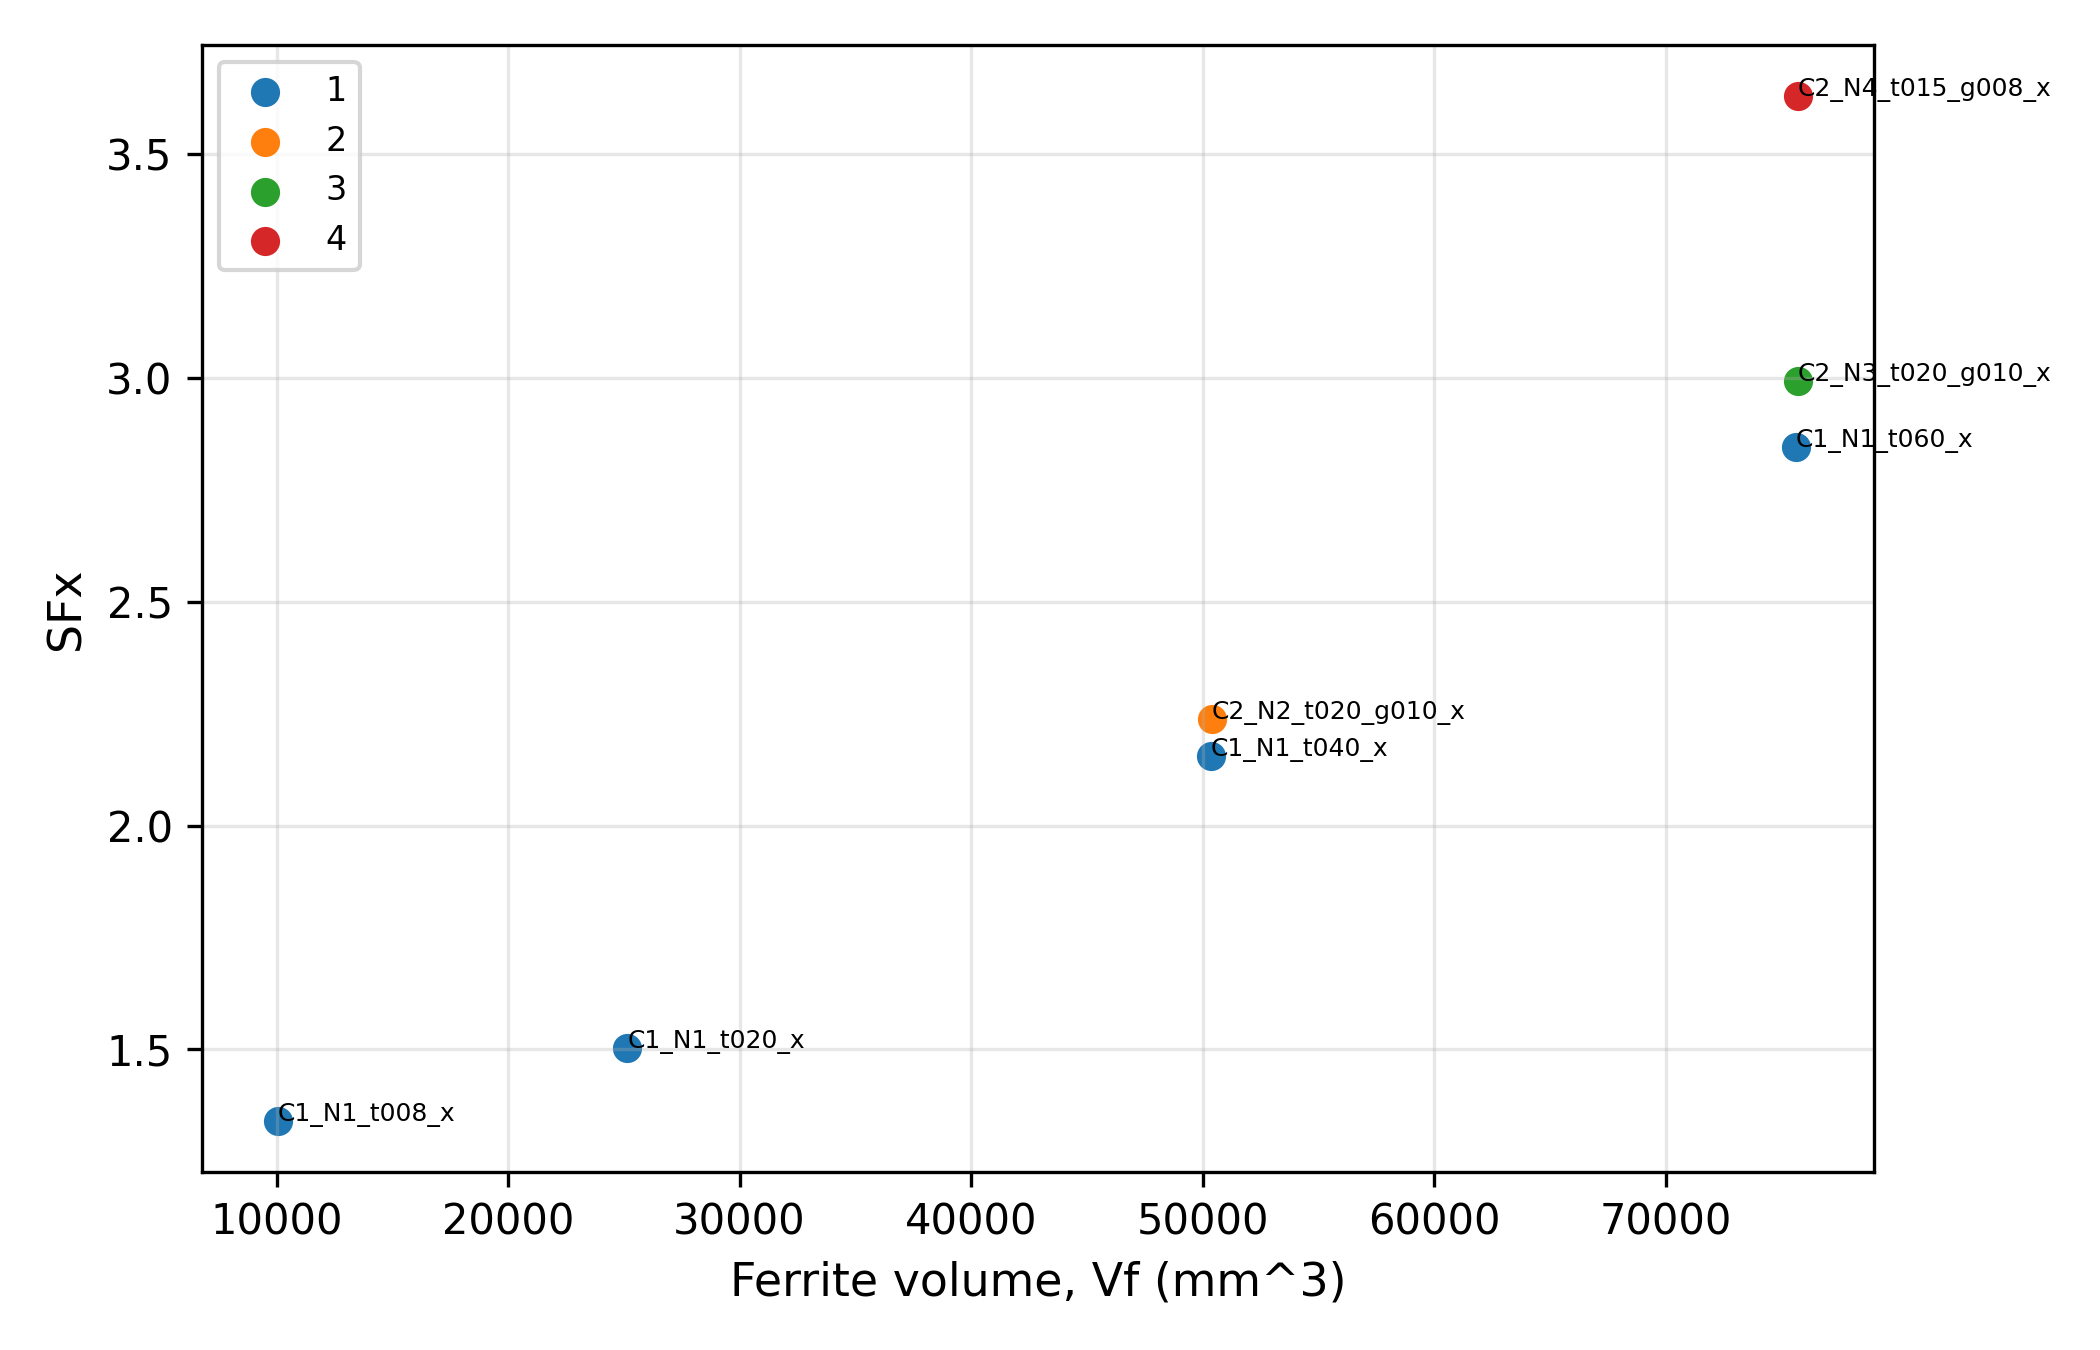
\includegraphics[width=\columnwidth]{../figures/Fig3_SFx_vs_Vf.png}
\caption{Transverse continuous-shell results: $\mathrm{SF}_x$ versus ferrite volume.}
\label{fig:sfxvf}
\end{figure}

\subsection{Fixed-Volume Comparison}

The cases C1\_N1\_t060\_x, C2\_N3\_t020\_g010\_x, and C2\_N4\_t015\_g008\_x have nearly equal ferrite volumes and allow a first comparison between thickness increase and multilayering under transverse continuous-shell conditions. Table~\ref{tab:fixedvolume} and Fig.~\ref{fig:fixedvolume} show that, among these validated transverse continuous-shell candidates, the four-layer case has the largest $\mathrm{SF}_x$, the largest $\eta_S^*$, and the smallest $\chi_H$. This ranking is not generalized to axial, segmented, or permeability-varied cases.

\begin{table}[!t]
\caption{Equal-Volume Transverse Comparison}
\label{tab:fixedvolume}
\centering
\footnotesize
\setlength{\tabcolsep}{2.5pt}
\begin{tabular}{lccccc}
\toprule
Case & $V_f$ & $\mathrm{SF}_x$ & IntH2 & $\eta_S^*$ & $\chi_H$ \\
 & (mm$^3$) & & (A$^2$m) & & \\
\midrule
C1\_N1\_t060\_x & 75624.4 & 2.845 & 4.649e-6 & 1.045 & 4.447e-6 \\
C2\_N3\_t020\_g010\_x & 75699.8 & 2.994 & 4.381e-6 & 1.095 & 3.995e-6 \\
C2\_N4\_t015\_g008\_x & 75714.9 & 3.629 & 4.160e-6 & 1.287 & 3.227e-6 \\
\bottomrule
\end{tabular}
\end{table}

\begin{figure}[!t]
\centering
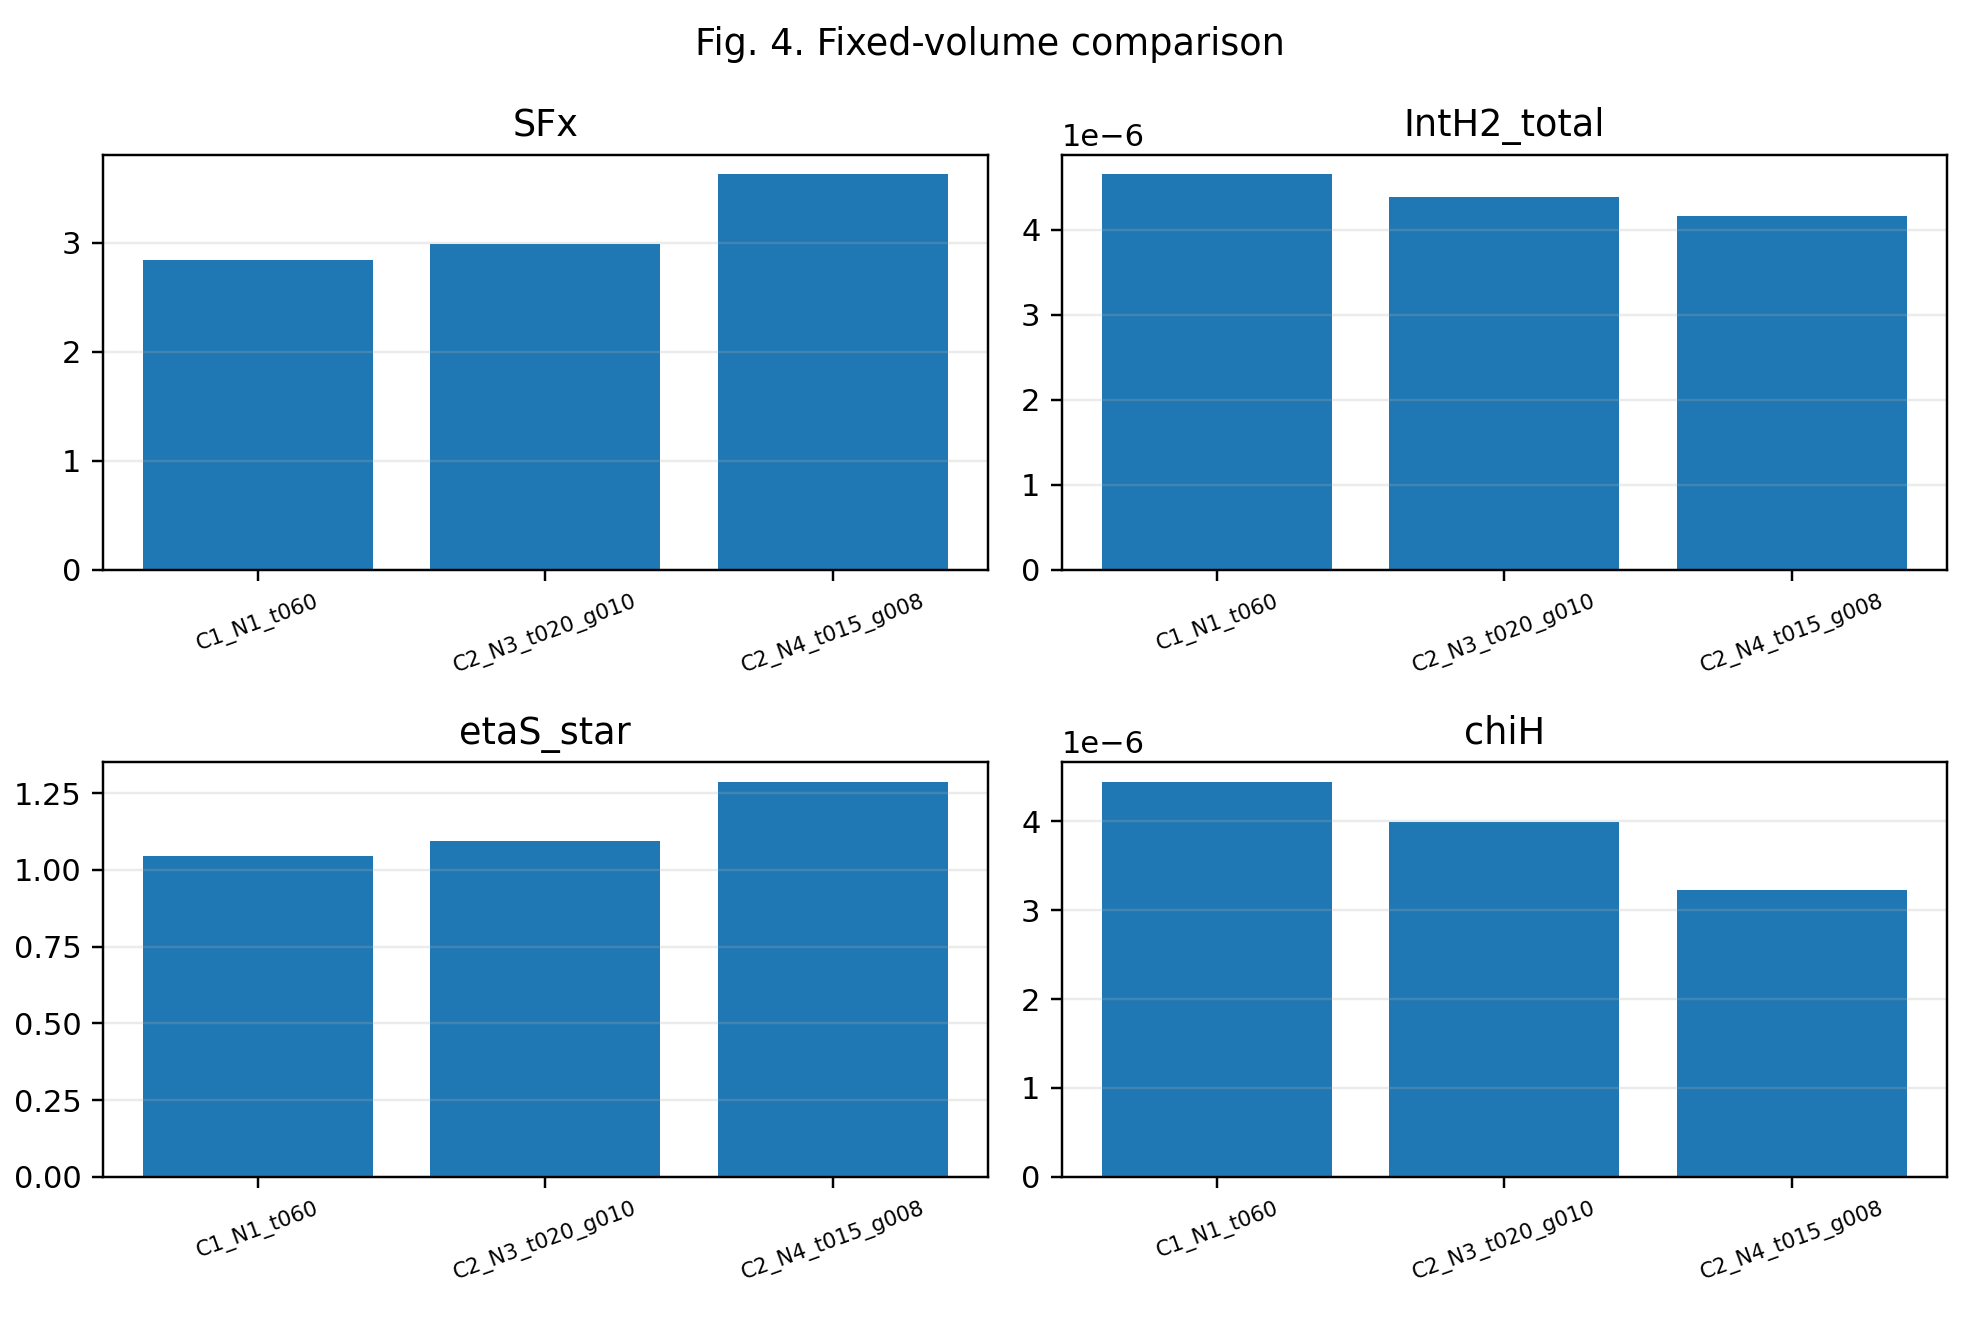
\includegraphics[width=\columnwidth]{../figures/Fig4_fixed_volume_comparison.png}
\caption{Equal-volume transverse comparison using $\mathrm{SF}_x$, IntH2, $\eta_S^*$, and $\chi_H$.}
\label{fig:fixedvolume}
\end{figure}

\subsection{Layer-Resolved IntH2 Distribution}

Layerwise IntH2 summation validation passed for all seven transverse continuous-shell cases. The multilayer fractions are listed in Table~\ref{tab:layerfraction} and plotted in Fig.~\ref{fig:layerfraction}. The four-layer case shows the largest fraction in the outermost layer under the present virtual-coil normalization. This observation is a geometry-dependent loss-integral distribution, not a measured magnetic-noise spectrum.

\begin{table}[!t]
\caption{Layerwise IntH2 Fractions for Multilayer Cases}
\label{tab:layerfraction}
\centering
\footnotesize
\begin{tabular}{lcccc}
\toprule
Case & L1 & L2 & L3 & L4 \\
 & (\%) & (\%) & (\%) & (\%) \\
\midrule
C2\_N2\_t020\_g010\_x & 49.4 & 50.6 & --- & --- \\
C2\_N3\_t020\_g010\_x & 25.7 & 36.1 & 38.2 & --- \\
C2\_N4\_t015\_g008\_x & 19.5 & 19.8 & 20.6 & 40.0 \\
\bottomrule
\end{tabular}
\end{table}

\begin{figure}[!t]
\centering
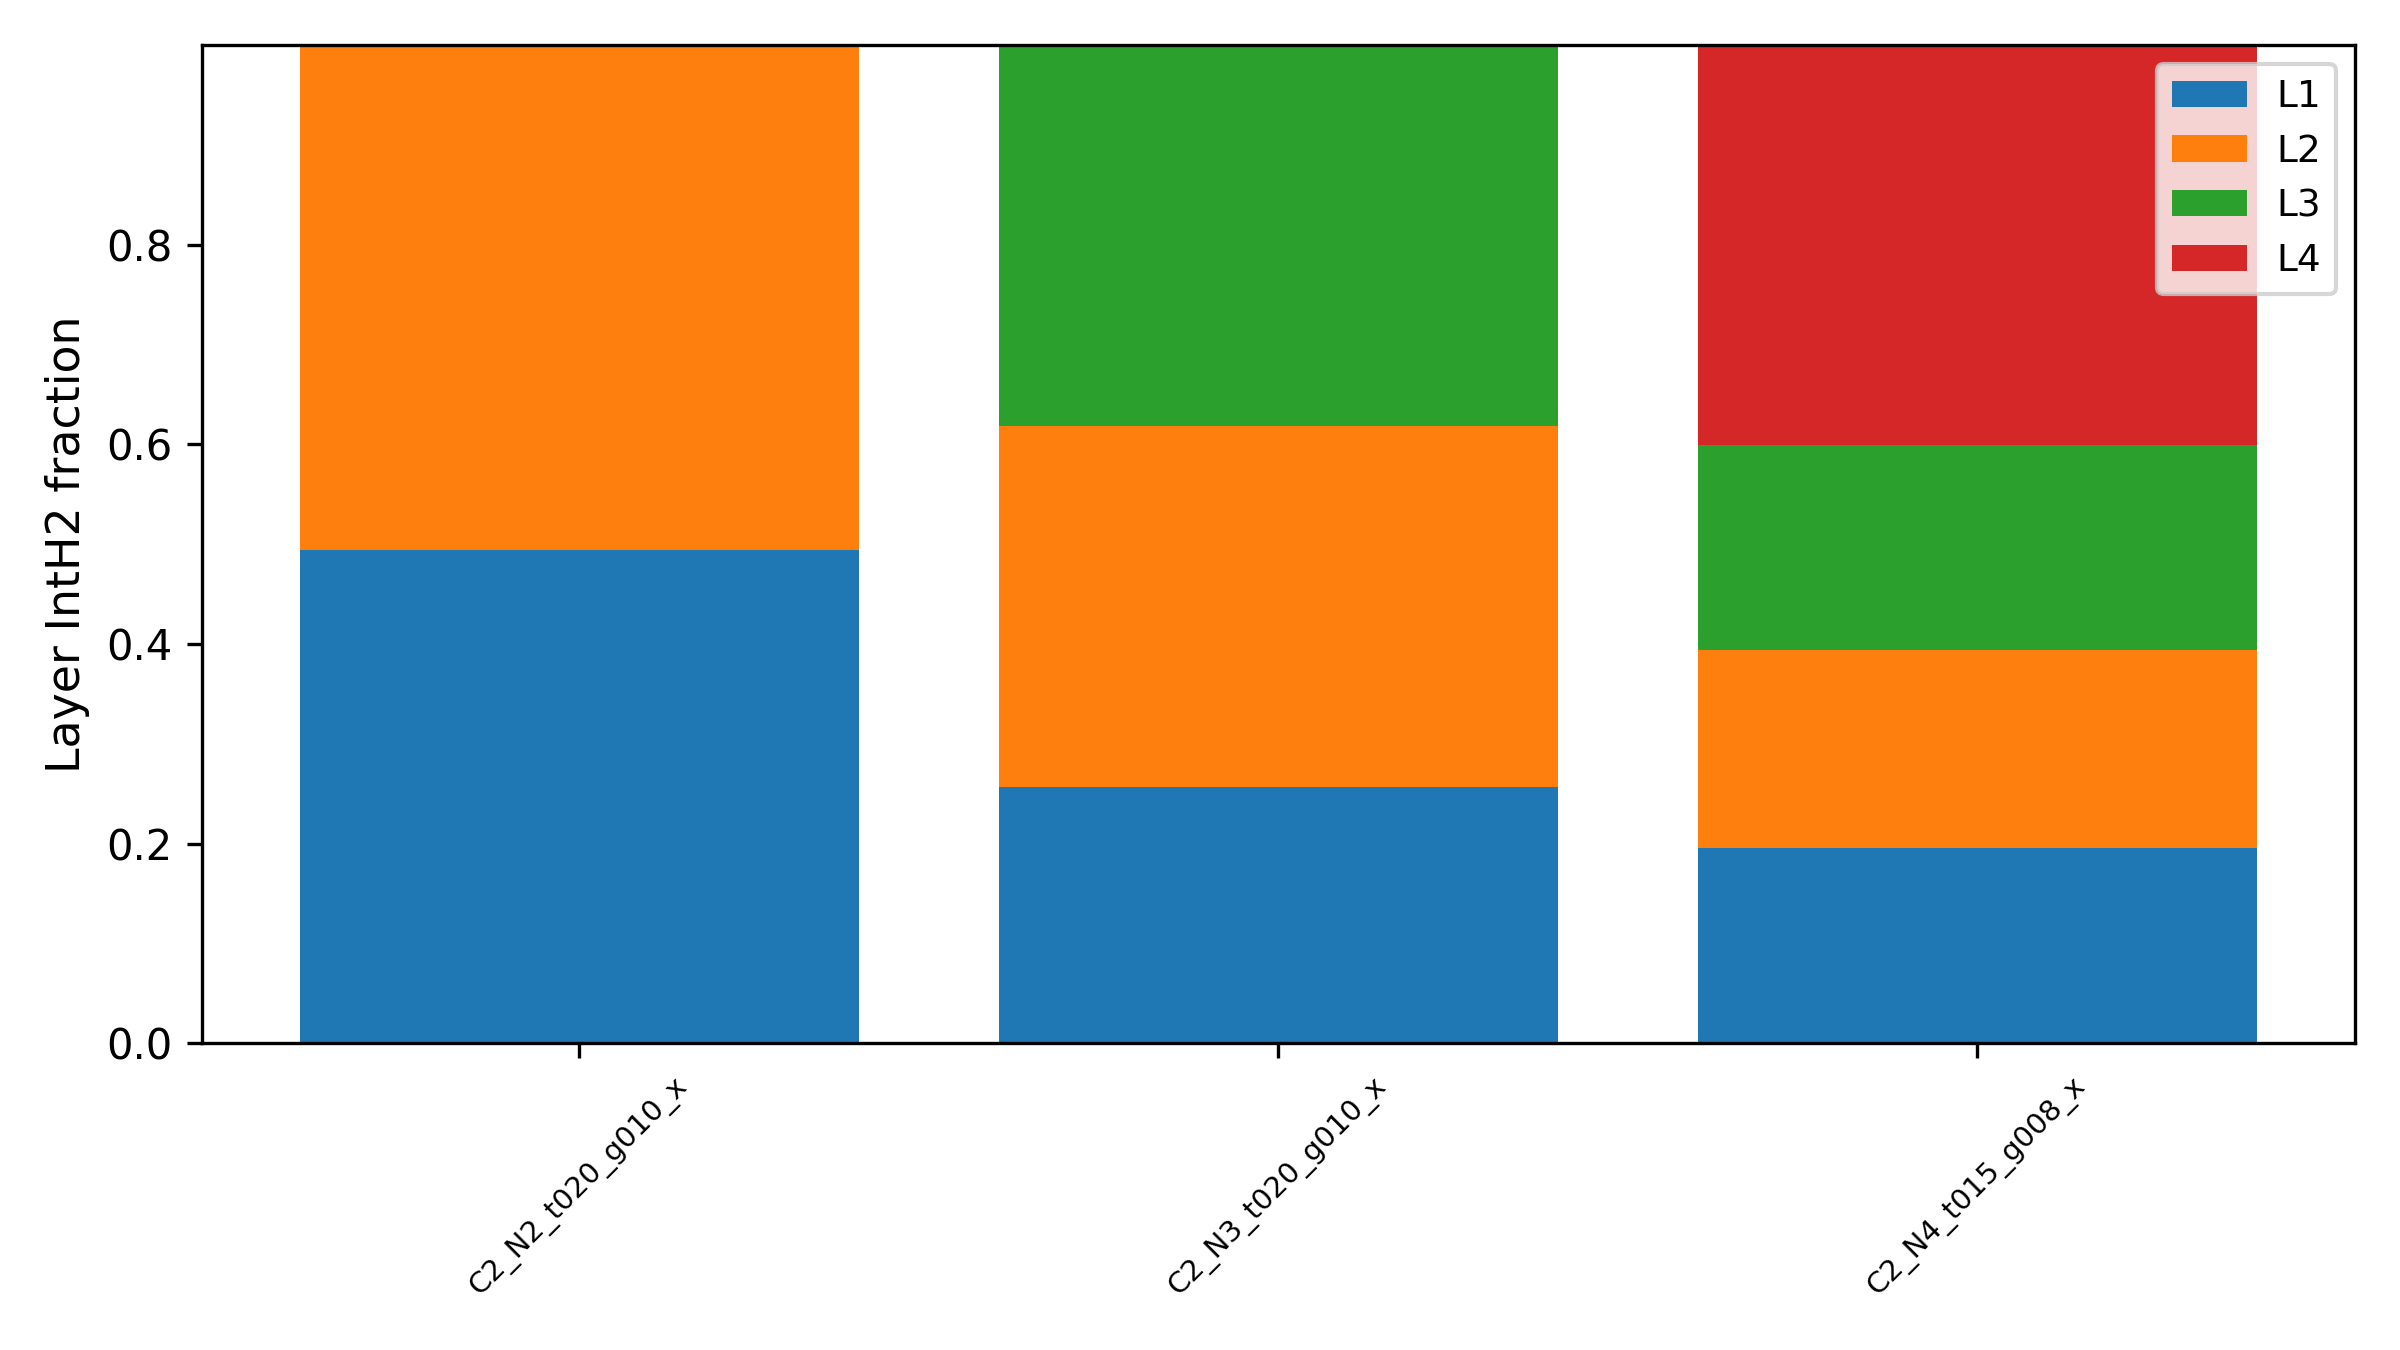
\includegraphics[width=\columnwidth]{../figures/Fig6_layerwise_IntH2_fraction.png}
\caption{Layer-resolved IntH2 fraction for validated multilayer transverse continuous-shell cases.}
\label{fig:layerfraction}
\end{figure}

\subsection{Mesh and Boundary-Domain Convergence}

Mesh convergence data are available for C1\_N1\_t008\_x and C2\_N4\_t015\_g008\_x. Medium-to-fine relative changes satisfy the numerical criteria for $B_{\mathrm{center},x}$, $\mathrm{SF}_x$, and IntH2, as summarized in Table~\ref{tab:mesh}. However, the exported mesh table does not yet include total element count, adaptive-pass count, or air-domain scale metadata. Therefore, the mesh trend is reported as a scalar convergence check, not as complete numerical-robustness verification. Boundary-domain convergence for C2\_N4\_t015\_g008\_x at 2R, 3R, and 5R air-domain scales remains unavailable and is excluded from robustness claims.

\begin{table*}[!t]
\caption{Mesh Convergence for the Representative Transverse Cases}
\label{tab:mesh}
\centering
\footnotesize
\setlength{\tabcolsep}{2.5pt}
\begin{tabular}{llcccccccc}
\toprule
Case & Mesh & Total & Across & Adaptive & Air & $B_{\mathrm{center},x}$ & $\mathrm{SF}_x$ & IntH2 & Rel. change \\
 & level & elements & thickness & passes & scale & (T) & & (A$^2$m) & (SFx/IntH2) \\
\midrule
C1\_N1\_t008\_x & coarse & --- & 1 & --- & --- & 9.265e-7 & 1.356 & 3.800e-6 & ---/--- \\
C1\_N1\_t008\_x & medium & --- & 3 & --- & --- & 9.375e-7 & 1.340 & 3.819e-6 & 1.19e-2/5.00e-3 \\
C1\_N1\_t008\_x & fine & --- & 5 & --- & --- & 9.375e-7 & 1.340 & 3.819e-6 & 1.72e-10/1.81e-10 \\
C2\_N4\_t015\_g008\_x & coarse & --- & 1 & --- & --- & 3.463e-7 & 3.629 & 4.160e-6 & ---/--- \\
C2\_N4\_t015\_g008\_x & medium & --- & 3 & --- & --- & 3.463e-7 & 3.629 & 4.160e-6 & 3.42e-10/8.17e-11 \\
C2\_N4\_t015\_g008\_x & fine & --- & 5 & --- & --- & 3.463e-7 & 3.629 & 4.160e-6 & 1.93e-10/4.33e-11 \\
\bottomrule
\end{tabular}
\end{table*}

\begin{figure}[!t]
\centering
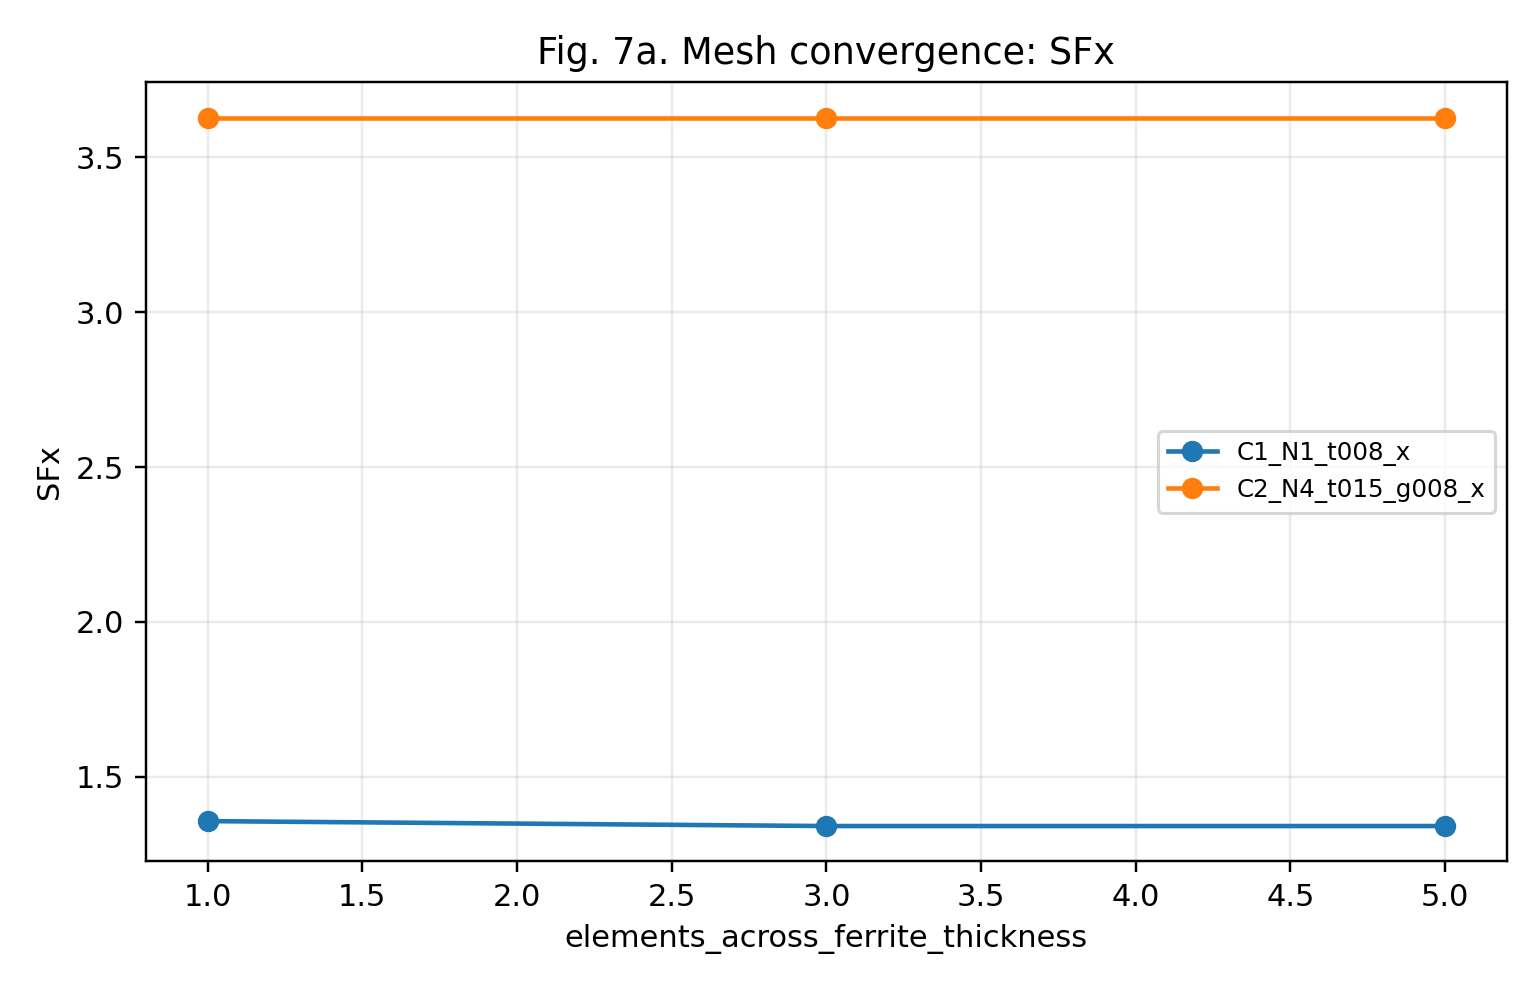
\includegraphics[width=\columnwidth]{../figures/mesh_convergence_sfx.png}
\caption{Mesh convergence of $\mathrm{SF}_x$ for the thinnest single-layer case and the four-layer candidate. Mesh metadata remain incomplete.}
\label{fig:meshsfx}
\end{figure}

\subsection{Axial Shielding Characterization}

The no-shield z-directed reference has passed direction validation. Shielded axial cases C1\_N1\_t060\_z, C2\_N3\_t020\_g010\_z, and C2\_N4\_t015\_g008\_z do not yet have valid shielded center-field exports. Therefore, $\mathrm{SF}_z$, $\mathrm{LeakageRatio}_z$, and $\mathrm{SF}_z/\mathrm{SF}_x$ are not reported as results, and the transverse $\mathrm{SF}_x$ ranking is not generalized to axial shielding.

\subsection{Segmented-Shell Correction}

Segmented aligned and staggered models are required to quantify manufacturable slot penalties. At present, segmented shielded exports are not available. The continuous-shell results should therefore be interpreted as idealized continuous-shell characterization, not as a validated segmented-assembly result.
The required segmented correction uses C2\_N4\_t015\_g008\_x with $N_{\mathrm{seg}}=12$ and $g_\phi=\SI{1.6}{mm}$ for both aligned and staggered slots. Because the aligned and staggered raw exports are not available, $\mathrm{SF}_{x,\mathrm{seg}}/\mathrm{SF}_{x,\mathrm{cont}}$ and $\mathrm{IntH2}_{\mathrm{seg}}/\mathrm{IntH2}_{\mathrm{cont}}$ are not reported.

\subsection{Permeability Sensitivity}

The validated transverse results use screening material parameters $\mu_r'=1000$ and $\sigma=\SI{0.01}{S/m}$. The required permeability comparison between C1\_N1\_t060\_x and C2\_N4\_t015\_g008\_x at $\mu_r'=500$, 1000, 2000, and 5000 is incomplete: only the $\mu_r'=1000$ baseline rows are available. Therefore, no robustness claim with respect to permeability variation is made, and no ranking stability is inferred.

\subsection{Field-Map Interpretation}

AEDT field-map exports for external-field $B$ distribution, flux lines, $H_{\mathrm{vc}}$, and $H_{\mathrm{vc}}^2$ contours are not yet available. The physical interpretation is therefore restricted to scalar quantities in the validated CSV exports. In particular, the high outer-layer IntH2 contribution is reported as an observed layerwise integral distribution, not as a confirmed field-mechanism explanation.

\section{Discussion}

The validated data show that the proposed characterization method can separate directional shielding, ferrite volume, and magnetic-noise-related loss indicators without relying on vector magnitude or unvalidated references. For low-noise magnetic instrumentation, this separation is important because an improved leakage-field attenuation does not by itself establish a lower shield-induced noise contribution. The present transverse results indicate that, among the equal-volume continuous-shell cases, distributing the same ferrite volume into the evaluated four-layer geometry increases $\mathrm{SF}_x$ and reduces $\chi_H$ relative to the evaluated single-layer and three-layer cases.

This ranking is directional and conditional. It applies to x-directed continuous-shell simulations using $\mu_r'=1000$ and the current geometry matrix. It is not extended to axial fields because the shielded z-directed exports are unavailable. This distinction matters for open-ended cylindrical shields, where end leakage can make axial and transverse shielding behave differently. Similarly, the continuous-shell result is not a manufacturable segmented-shell result until aligned and staggered slot corrections are exported and validated.

The IntH2 results should be read as magnetic-noise-related loss indicators, not measured magnetic noise. The layerwise IntH2 fractions show that the outer layer carries the largest fraction in the four-layer case, but the AEDT field-map exports needed to explain this distribution are not yet available. Therefore, the discussion is limited to the observed scalar integral distribution. Detailed physical claims about flux redistribution or local virtual-coil field concentration should be added only after external-field and $H_{\mathrm{vc}}^2$ contours are exported.

The material-parameter dependence is also unresolved. Only $\mu_r'=1000$ is validated in the present comparison, so the equal-volume ranking cannot yet be called robust to permeability variation. The next required sensitivity sweep at $\mu_r'=500$, 2000, and 5000 should be used to determine whether the higher $\mathrm{SF}_x$ and lower $\chi_H$ of the four-layer case persist under plausible ferrite-property variation.

\section{Conclusion}

A measurement-oriented characterization method for multilayer thin-ferrite cylindrical shields has been established and applied to validated transverse continuous-shell AEDT exports. The method uses a passed no-shield directional reference, component-based $\mathrm{SF}_x$, layer-resolved IntH2 checks, exact ferrite-volume calculation, and unit-consistent auxiliary metrics. For the seven validated transverse continuous-shell candidates, the equal-volume four-layer design gives the highest $\mathrm{SF}_x$ and the lowest IntH2-normalized auxiliary loss indicators among the candidates evaluated. Mesh convergence checks for the thinnest single-layer and selected four-layer cases support the reported scalar values, but the mesh metadata are incomplete and boundary-domain convergence has not yet been completed.

The current conclusions are limited to transverse continuous-shell cases with screening material parameters. They do not establish axial performance, segmented-assembly performance, complete numerical robustness, permeability-variation robustness, or a final instrument-level recommendation. IntH2 is treated only as a magnetic-noise-related loss indicator; absolute magnetic-noise spectra require measured $\mu_r''(f)$ and experimental validation.

\appendices
\section{Prototype SF Measurement Note}
\label{app:prototype}
No experimental shielding-factor data are included in the present manuscript. A future prototype measurement should use a calibrated Helmholtz or triaxial coil system and a calibrated magnetic sensor, with $B_0$ and $B_{\mathrm{center}}$ evaluated from the same directional component used in the FEM definition. For independent measurements,
\begin{equation}
\frac{u(\mathrm{SF}_{q,\mathrm{exp}})}{\mathrm{SF}_{q,\mathrm{exp}}}
=
\sqrt{
\left[\frac{u(B_{0,q})}{B_{0,q}}\right]^2+
\left[\frac{u(B_{\mathrm{center},q})}{B_{\mathrm{center},q}}\right]^2
}.
\label{eq:uncertainty}
\end{equation}
For correlated measurements,
\begin{equation}
u_r^2(\mathrm{SF}_{q,\mathrm{exp}})=
u_r^2(B_0)+u_r^2(B_{\mathrm{center}})
-2\rho u_r(B_0)u_r(B_{\mathrm{center}}).
\label{eq:corruncertainty}
\end{equation}

\section*{Acknowledgment}
Funding, facilities, and collaborator acknowledgments should be added before submission.

\begin{thebibliography}{31}

\bibitem{ref1}
J.~C.~Allred, R.~N.~Lyman, T.~W.~Kornack, and M.~V.~Romalis,
``High-sensitivity atomic magnetometer unaffected by spin-exchange relaxation,''
\textit{Phys. Rev. Lett.}, vol.~89, no.~13, Sep.~2002, Art.~no.~130801.

\bibitem{ref2}
I.~K.~Kominis, T.~W.~Kornack, J.~C.~Allred, and M.~V.~Romalis,
``A subfemtotesla multichannel atomic magnetometer,''
\textit{Nature}, vol.~422, no.~6932, pp.~596--599, Apr.~2003.

\bibitem{ref3}
M.~P.~Ledbetter, I.~M.~Savukov, V.~M.~Acosta, D.~Budker, and M.~V.~Romalis,
``Spin-exchange-relaxation-free magnetometry with Cs vapor,''
\textit{Phys. Rev. A}, vol.~77, no.~3, Mar.~2008, Art.~no.~033408.

\bibitem{ref4}
S.~Baillet,
``Magnetoencephalography for brain electrophysiology and imaging,''
\textit{Nature Neurosci.}, vol.~20, no.~3, pp.~327--339, Mar.~2017.

\bibitem{ref5}
T.~E.~Chupp, P.~Fierlinger, M.~J.~Ramsey-Musolf, and J.~T.~Singh,
``Electric dipole moments of atoms, molecules, nuclei, and particles,''
\textit{Rev. Mod. Phys.}, vol.~91, no.~1, Jan.~2019, Art.~no.~015001.

\bibitem{ref6}
T.~J.~Sumner, J.~M.~Pendlebury, and K.~F.~Smith,
``Conventional magnetic shielding,''
\textit{J. Phys. D: Appl. Phys.}, vol.~20, no.~9, pp.~1095--1101, Sep.~1987.

\bibitem{ref7}
V.~Kelha, J.~Pukki, R.~Peltonen, A.~Penttinen, R.~Ilmoniemi, and J.~Heino,
``Design, construction, and performance of a large-volume magnetic shield,''
\textit{IEEE Trans. Magn.}, vol.~18, no.~1, pp.~260--270, Jan.~1982.

\bibitem{ref8}
I.~Altarev \textit{et al.},
``A magnetically shielded room with ultra low residual field and gradient,''
\textit{Rev. Sci. Instrum.}, vol.~85, no.~7, Jul.~2014, Art.~no.~075106.

\bibitem{ref9}
S.-K.~Lee and M.~V.~Romalis,
``Calculation of magnetic field noise from high-permeability magnetic shields and conducting objects with simple geometry,''
\textit{J. Appl. Phys.}, vol.~103, no.~8, Apr.~2008, Art.~no.~084904.

\bibitem{ref10}
H.~B.~Dang, A.~C.~Maloof, and M.~V.~Romalis,
``Ultrahigh sensitivity magnetic field and magnetization measurements with an atomic magnetometer,''
\textit{Appl. Phys. Lett.}, vol.~97, no.~15, Oct.~2010, Art.~no.~151110.

\bibitem{ref11}
D.~Ma \textit{et al.},
``A novel low-noise mu-metal magnetic shield with winding shape,''
\textit{Sens. Actuators A, Phys.}, vol.~346, Oct.~2022, Art.~no.~113884.

\bibitem{ref12}
T.~W.~Kornack, S.~J.~Smullin, S.-K.~Lee, and M.~V.~Romalis,
``A low-noise ferrite magnetic shield,''
\textit{Appl. Phys. Lett.}, vol.~90, no.~22, May~2007, Art.~no.~223501.

\bibitem{ref13}
D.~Ma \textit{et al.},
``Parameter modeling analysis of a cylindrical ferrite magnetic shield to reduce magnetic noise,''
\textit{IEEE Trans. Ind. Electron.}, vol.~69, no.~1, pp.~991--998, Jan.~2022.

\bibitem{ref14}
J.~Lu \textit{et al.},
``Study of magnetic noise of a multi-annular ferrite shield,''
\textit{IEEE Access}, vol.~8, pp.~40918--40924, 2020.

\bibitem{ref15}
B.~Sun \textit{et al.},
``Correlating the microstructure of Mn--Zn ferrite with magnetic noise for magnetic shield applications,''
\textit{Ceram. Int.}, vol.~49, no.~8, pp.~11960--11967, Apr.~2023.

\bibitem{ref16}
B.~Sun, D.~Ma, X.~Fang, Y.~Xue, J.~Lu, H.~Chen, M.~Zhang, H.~Wei, B.~Han, and Y.~Zhai,
``Suppression of magnetic noise and field in cubic low-noise ferrite magnetic shields,''
\textit{IEEE Trans. Instrum. Meas.}, vol.~73, pp.~1--10, 2024, Art.~no.~1501810.

\bibitem{ref17}
J.~Lu \textit{et al.},
``Effect of gaps on magnetic noise of cylindrical ferrite shield,''
\textit{J. Phys. D: Appl. Phys.}, vol.~54, no.~25, Jun.~2021, Art.~no.~255002.

\bibitem{ref18}
R.~Kubo,
``The fluctuation-dissipation theorem,''
\textit{Rep. Prog. Phys.}, vol.~29, no.~1, pp.~255--284, Jan.~1966.

\bibitem{ref19}
C.~Liu \textit{et al.},
``Investigation on the effects of micro-vibration on the atomic comagnetometer,''
\textit{IEEE Trans. Instrum. Meas.}, vol.~72, 2023, Art.~no.~9511711.

\bibitem{ref20}
P.~Dutta and P.~M.~Horn,
``Low-frequency fluctuations in solids: $1/f$ noise,''
\textit{Rev. Mod. Phys.}, vol.~53, no.~3, pp.~497--516, Jul.~1981.

\bibitem{ref21}
K.~Yang \textit{et al.},
``Improved measurement of the low-frequency complex permeability of ferrite annulus for low-noise magnetic shielding,''
\textit{IEEE Access}, vol.~7, pp.~126059--126065, 2019.

\bibitem{ref22}
K.~Yang \textit{et al.},
``Minimizing magnetic fields of the low-noise MnZn ferrite magnetic shield for atomic magnetometer,''
\textit{J. Phys. D: Appl. Phys.}, vol.~55, no.~1, Jan.~2022, Art.~no.~015003.

\bibitem{ref23}
Z.~Xu, Z.~Zhang, B.~Wu, H.~Wang, X.~Kong, and M.~Wang,
``A study of enclosed magnetic shielding room by simulation,''
\textit{IEEE Trans. Appl. Supercond.}, vol.~31, no.~8, pp.~1--5, Nov.~2021.

\bibitem{ref24}
X.~Xu, L.~Wang, W.~Liu, and Z.~Zhao,
``Theoretical modeling and characterization of equivalent magnetic properties in laminated composite magnetic shielding,''
\textit{Measurement}, vol.~251, 2025, Art.~no.~117237.

\bibitem{ref25}
\textit{Cores Made of Soft Magnetic Materials---Measuring Methods---Part 2: Magnetic Properties at Low Excitation Level}, IEC 62044-2, 2005.

\bibitem{ref26}
TDK Corporation,
``Mn--Zn ferrite material characteristics: PC95 and related Mn--Zn ferrite grades,''
product catalog, accessed May~2026. [Online]. Available: \url{https://product.tdk.com/system/files/dam/doc/product/ferrite/ferrite/ferrite-core/catalog/ferrite_mn-zn_material_characteristics_en.pdf}

\bibitem{ref27}
A.~Mager,
``Magnetic shields,''
\textit{IEEE Trans. Magn.}, vol.~6, no.~1, pp.~67--75, Mar.~1970.

\bibitem{ref28}
K.~Nagashima, I.~Sasada, and K.~Tashiro,
``High-performance bench-top cylindrical magnetic shield with magnetic shaking enhancement,''
\textit{IEEE Trans. Magn.}, vol.~38, no.~5, pp.~3335--3337, Sep.~2002.

\bibitem{ref29}
J.~M.~G.~D.~K.~O'Connell, J.~M.~Brown, and T.~W.~Kornack,
``Technique for high axial shielding factor performance of large-scale, thin, open-ended, cylindrical Metglas magnetic shields,''
arXiv:1107.2625, 2011.

\bibitem{ref30}
J.~Fang, S.~Wan, J.~Qin, and Y.~Chen,
``A novel method for in-situ measuring the static shielding factor of a magnetic shield,''
\textit{Measurement}, vol.~170, 2021, Art.~no.~108718.

\bibitem{ref31}
T.~Brys \textit{et al.},
``Magnetic field stabilization for magnetically shielded volumes by external field coils,''
\textit{J. Appl. Phys.}, vol.~116, no.~8, 2014, Art.~no.~084903.

\end{thebibliography}

\end{document}
